\section{Performance implications}
In our evaluations we seek to answer whether cooperative scheduling can meaningfully improve overall performance. Unless otherewise noted, we focus on overall system throughput. The workloads that might benefit most from our proposal--batch data analytics--motivate this choice.

\begin{figure*}
\centering
\begin{tabular}{|l|l|c|c|c|c|c|}
\hline
\multirow{2}{*}{\textbf{Name}} & \multirow{2}{*}{\textbf{Application domain}} & \multicolumn{2}{|c|}{\textbf{Parallelization}} & \multirow{2}{*}{\textbf{Working set}} & \multicolumn{2}{|c|}{\textbf{Data usage}} \\
& & \textbf{Model} & \textbf{Granularity} & & \textbf{Sharing} & \textbf{Exchange} \\
\hline
\textbf{\texttt{\text{*}blackscholes}} & Financial analysis & data-parallel & coarse & small & low & low \\
\hline
\textbf{\texttt{bodytrack}} & Computer vision & data-parallel & medium & medium & high & medium \\
\hline
\textbf{\texttt{\text{*}canneal}} & Engineering & unstructured & fine & unbounded & high & high \\
\hline
\textbf{\texttt{\text{*}dedup}} & Enterprise storage & pipeline & medium & unbounded & high & high \\
\hline
\textbf{\texttt{facesim}} & Animation & data-parallel & coarse & large & low & medium \\
\hline
\textbf{\texttt{ferret}} & Similarity search & pipeline & medium & unbounded & high & high \\
\hline
\textbf{\texttt{\text{*}fluidanimate}} & Animation & data-parallel & fine & large & low & medium \\
\hline
\textbf{\texttt{freqmine}} & Data mining & data-parallel & medium & unbounded & high & medium \\
\hline
\textbf{\texttt{\text{*}streamcluster}} & Data mining & data-parallel & medium & medium & low & medium \\
\hline
\textbf{\texttt{\text{*}swaptions}} & Financial analysis & data-parallel & coarse & medium & low & low \\
\hline
\textbf{\texttt{vips}} & Media processing & data-parallel & coarse & medium & low & medium \\
\hline
\textbf{\texttt{x264}} & Media processing & pipeline & coarse & medium & high & high \\
\hline
\end{tabular}
\label{table:parsec-apps}
\captionof{table}{Applications annotated with a * have been integrated with the \mech{} client library. This is a qualitative summary of all the workloads in the PARSEC benchmark. PARSEC workloads were chosen to cover different application domains, parallel models and runtime behaviors.~\cite{bienia2012characteristics}}
\end{figure*}
\subsection{Prototype implementation}
When implementing our prototype, we opted for simpler designs and heuristics. The message bus, scheduler, and client library together comprise fewer than 2000 lines of C and C++. Thanks to the design of the PARSEC benchmark suite, we were able to integrate the client library into many of the benchmark applications with fewer than 100 lines of modified code. To simplify communication among components, we use shared memory and locks, allowing us to forgo message queues or additional threads to maintain communication.

Although we implemented more complex mechanisms, we were able to demonstrate strong results using the most basic configuration. In the following experiments, the scheduler only polls the system-wide run queue and ignores any other system or application-specific data. Given that the target workloads are CPU-intensive, using thread contention as a proxy for resource contention is reasonable. Despite this simplicity, however, the application implicitly gives the scheduler a lot of information by registering as a client. Most importantly, the application signals that it is capable of dynamic run-time parallelism and is willing to follow directives from the scheduler.

During run-time, the scheduler provides applications with a recommended number of threads to create on start. We assume that applications are well-behaved, but it would not be difficult to implement punitive measures.

\subsection{Experimental environment}
We conducted experiments on four different machine types: a quad-core desktop (8 hardware threads), a dual-socket 9-core c4.8xlarge Amazon EC2 instance (36 vCPUs), a 4-socket 10-core workstation (80 hardware threads), and a cluster with many 68-core machines (272 hardware threads). Although our findings are consistent across machines, we choose to present results from the 68-core machines to illustrate the challenges introduced by these manycore chips.

The cluster is part of a research installation generously maintained by the Intel$^{\tiny{\textregistered}}$ Corporation and features 256 nodes each equipped with an Intel Xeon Phi\texttrademark CPU (Model 7250). Each Xeon Phi\texttrademark has 68 physical 1.4GHz cores with 4 hardware threads per core. Each physical core has 32K of L1d and L1i cache and shares a 1024K L2 cache with one other core. The CPU can be configured in several ways. First, we use the fully symmetric NUMA topology as opposed to the quadrant mode to simplify the profiling and debugging process. Second, we use the 16GB on-package memory as a large last-level cache rather than use it as ultra-fast memory so our results are more generally applicable to less sophisticated hardware.

\subsection{Benchmark applications}
To evaluate our \mech{}, we use a popular parallel application suite, PARSEC~\cite{bienia2008parsec}, to generate a large number of diverse workloads spanning several classes of parallel programs and problem domains (see Table 1). After integrating the client library into each application, we control their levels of parallelism as they enter the system. For six applications (see starred applications in Tabl 1), we also instrumented the capabiltiy to dynamically adjust parallelism during program execution. However, in experiments, we found that the overhead of such a design is only justified for longer-running applications residing with unpredictably busy neighbors.

\subsection{Baseline comparisons}
In order to create an apples-to-apples comparison unencumbered by differences in implementation, we chose to evaluate the workloads using two existing thread libraries with and without cooperation. We use the Pthreads standard as an example of lower-level parallel programming and the Intel$^{\tiny{\textregistered}}$ Thread Building Blocks (TBB) library as an example of a sophisticated industrial-grade library. Eleven of the twelve PARSEC benchmark applications are implemented using Pthreads and five also have TBB implementations.

\subsection{Generating workloads}
In order to compare performance, we create several hundred randomly-generated workloads by drawing samples from the set of benchmark applications. We focus our attention on constant load scenarios as these are most advantageous to the existing parallel programming libraries. More dynamic loads are amenable to our approach since they offer many opportunities to change an application's parallelism to adjust to new circumstances.

We run each workload with Pthreads and TBB in their normal use case and as part of a cooperative environment. For each of these four cases, we run for several levels of cotenancy, modeled by some constant number of simultaneously running applications.

\subsection{Coordinating with \mech{}s}
\begin{figure*}[t!]
    \centering
    \begin{subfigure}[t]{0.5\textwidth}
        \centering
        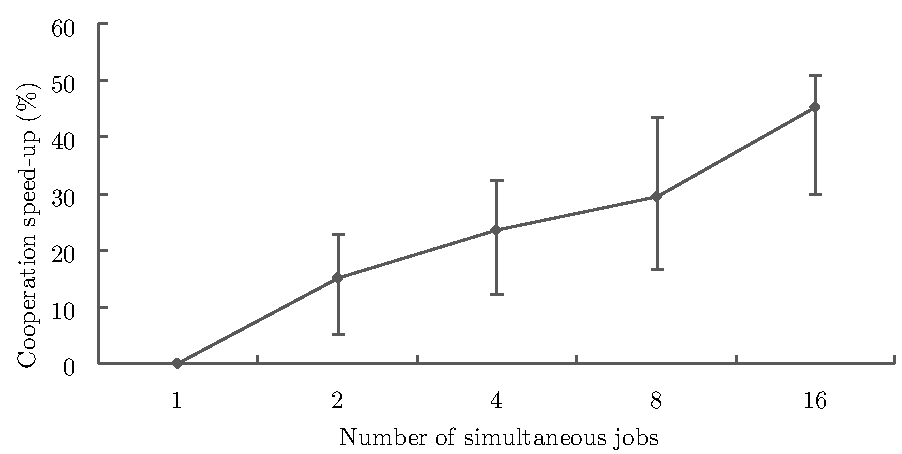
\includegraphics[width=8cm,height=4cm]{fig/randomized-pthreads.pdf}
        \caption{Pthreads implementation}
        \label{fig:pthread}
    \end{subfigure}%
    ~ 
    \begin{subfigure}[t]{0.5\textwidth}
        \centering
        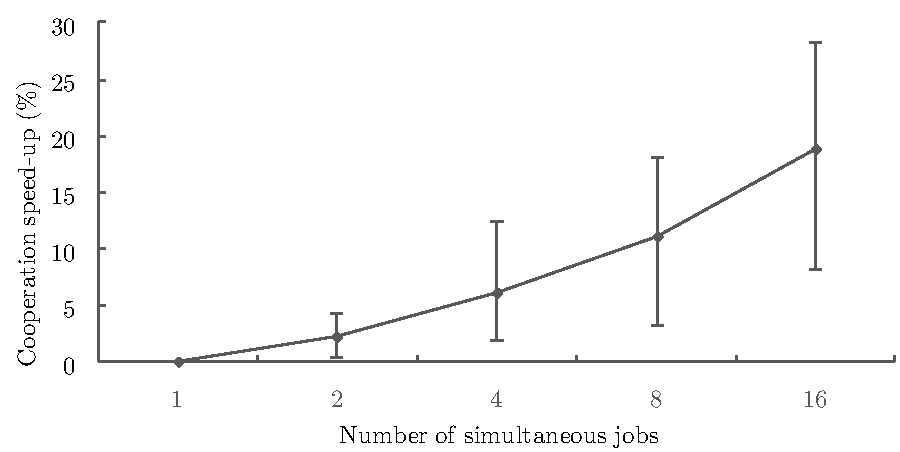
\includegraphics[width=8cm,height=4cm]{fig/randomized-tbb.pdf}
        \caption{Intel$^{\mbox{\tiny\textregistered}}$ Threading Building Blocks (TBB) implementation}
        \label{fig:tbb}
    \end{subfigure}
    \label{fig:randomized}
    \caption{The benefit from cooperation increases with contention. Each observation is 100 jobs (100 tasks each) run both with and without cooperation. The line represents the mean throughput (time to job completion) while error bars represent the maximum and minimum speed-ups we observed. Of note, we did not observe our mechanism harming performance.}
\end{figure*}
We show our main results in Figure 5. The pair of figures show the same experiments for Pthreads and TBB. The vertical axis indicates how much faster the cooperative approach completed workloads relative to the pre-emptive approach on the same workload. The line shows mean speed-up for the specified load level and the error bars show the maximum and minimum observed speed-ups.

There are two important observations. First, we did not observe in any scenario where cooperating led to a worse outcome. Second, cooperation improves performance to a greater extent with increasing contention. We were able to achieve such a result with a simple design because our workload has a number of structural features (e.g., CPU-intensive, parallel structure) that lend themselves to cooperation.

% \subsection{Characterizing results}



% We want to discuss the following and map to real-world workloads
% \begin{itemize}
% \item What we are good for: large-scale batch compute for big data. Individual latency doesn't matter; about throughput. Make sure to address the fact that analytics framework (e.g., spark) do parallelization at task / process level
% \item What we don't really affect
% \item What we are bad for
% \end{itemize}

% \subsection{Measure overhead}
% Don't compare against original implementation since that's apples and oranges. But here it is anyway for overhead purposes.
